\cleartooddpage[\thispagestyle{empty}]
\chapter{Hemodynamic Flow Vortex Identification}\label{CHAPTER3}

The assessment of disturbed hemodynamic patterns is known to have an impact on the origin and national history of IAs \cite{weir2002unruptured,brisman2006cerebral}. From a clinical perspective, phase-contrast magnetic resonance imaging (PC-MRI) or Phase-contrast magnetic resonance angiography (PC-MRA) has been used to assess flow characteristics in the vasculature \textit{in-vivo} \cite{benndorf1996intraaneurysmal,meckel2008vivo}. Yet, determining flow details in and around IAs has proven difficult with PC-MRI/PC-MRA. The complex, disturbed patterns of aneurysmal flow results in incoherent velocites (at the sub-grid level) and these specific characteristics cannot be resolved by a typical "averaged" velocity measurement at the relatively large resolution in medical imaging (\textit{at 1-mm scale}). The consequence of this sub-grid limitation, clinical hemodynamic flow measurements may be impacted by errors and potential flow artifacts which adversely affect the accuracy of PC-MRI/PC-MRA results \cite{strater20184d,meckel2008vivo}. In parallel to research efforts of assessing MR flow imaging in and around IAs to determine rupture characteristics, blood flow simulated from "patient-specific" computational fluid dynamics (CFD) simulations \cite{steinman2002image} have also garnered interest by the clinical and research community \cite{xiang2011hemodynamic,cebral2011association}. CFD simulation data has an initial advantage over MRI derived data in that a high degree of control of both desired data resolution, as well as data quality (lack of imaging errors and flow artifacts) can be maintained. The development of novel flow measurement techniques can be initially tested and refined on data free from errors which may confound initial findings.

Assessment of hemodynamic conditions from CFD simulations has brought about a number of potential parameters that correlate to IA rupture risk: wall shear stress \cite{baek2009flow}, oscillatory shear index \cite{steinman2003image}, flow impingement \cite{cebral2011association}, and flow stability \cite{byrne2014quantifying}. As mentioned in the focus of flow stability, Bryne et al. \cite{byrne2014quantifying} found that aneurysmal flow flow spatial complexity and temporal stability is closely correlated with IA rupture. Yet this methodology only relies on qualitative assessment of the centroid-most region of vortex patterns (vortex core), giving less insight on the broader structural changes to vortices. Expanding upon the idea of vortex analysis to identify, and quantify changes to, the broader structural characteristics of vortices may give additional insight into conditions that can be linked to IA rupture potential.

In an initial study, the development of an alternative technique for vortex analysis (expanding upon vortex core analysis) was investigated to assess the presence, destruction and spatialtemporal characteristics of vortices within an IA \cite{sunderland2016vortex}. This image processing algorithm expanded upon two established vortex identification methods, the \textit{Q}-criterion \cite{hunt1988eddies} and $\lambda_2$ \cite{jeong1995identification} methods, to identify and assess the broader aspects of vortices as opposed to solely identifying the vortex core. Subsequent studies investigated the use of a vortex identification methodology based on the Shannon's entropy (CITATION NEEDED) as an alternative identification metric not wholly reliant upon vortex core identification. 

Due to the differences between traditional CFD data resolution (high) and MRI derived flow data (lower resolution), the identification methods were based on velocity data on a rectilinear grid, and the susceptibility of changes to vortex identification outcomes were tested under a range of grid resolutions. Additionally, variations to methodological outputs were tested under a range of chosen threshold values (dependent on the method and will be explained in Section NEED THE SECTION). The vulnerability of a methodology to significant changes in outcomes with minimal changes to methodological threshold values would have the potential to result in broad variations to research findings if thresholds were to be applied to a wide array of studies. Toward this end, the primary focus of this work was to explore analyzing the spatiotemporal characteristics of hemodynamic vortex structures as a possible means to compliment future assessment of IA rupture potential.  

\section{Materials and Methods}\label{CHAPTER3_SECTION1}
\subsection{Modeling of "Patient-specific" Vasculature}\label{CHAPTER3_SECTION1_SUBSECTION1}

Medical imaging scans of ten (10) patient's vasculature structure were arbitrarily selected from an internal database: five patients with a single bifurcation aneurysm, and five with a single sidewall aneurysm. Models were located within the internal carotid artery or the basilar artery. A commercially available image segmentation package (Mimics Innovation Suite, version 17, Materialise Inc. Leuven, Belgium) was used to reconstruct the vascular surface from digital subtraction angiography (DSA) scans, resulting in 'patient-specific' vascular structures. For all cases, the longest available upstream vessel section proximal to the aneurysm was left intact to maintain as much of the patient vessel geometry as possible. Surface irregularities were manually removed using the localized smoothing capability in the commercially available computer aided design (CAD) 3-matic software (Version 9, Materialize Inc., Leuven, Belgium). Additionally, a $1^{st}$ order Laplacian smoothing filter was used to perform a global smoothing to the vessel structure, reducing surface irregularities while preserving the vascular geometry. Cylindrical flow extensions (6 times the inlet vessel diameter) were added to each model using the open-source Vascular Modeling Toolkit (VMTK) software (version 1.2). The addition of vessel extensions help reduce the effects of inlet, plug-flow flow on hemodynamic characteristics \cite{poethke2009cerebral}.

\subsection{Mesh Generation}\label{CHAPTER3_SECTION1_SUBSECTION2}
Processed vascular surface structures were converted into an unstructured, 3D, tetrahedralized volumetric mesh using an open-source mesh generator, Tetgen (version 1.4.2) \cite{si20113d}. The mesh generation process was done by an in-house Python script derived from the VMTK program. Approximately, 1 million computing cells were used per case, with the average mesh size as 0.0022-mm$^{3}$.

\subsection{CFD Simulation}\label{CHAPTER3_SECTION1_SUBSECTION3}
To compute fluid velocity data in and around the IA, the time-dependent incompressible, 3D Navier-Stokes equations was  (THERE NEEDS TO BE AN ADJECTIVE HERE....CHECK RECENT PAPERS) solved using two CFD solvers: a commercial CFD solved (version 14.0, ANSYS-FLUENT Inc., Lebanon, NH) and a research prototype CFD solver (version 4.0, Siemens Medical Solution Inc., IL). Details on the Navier-Stokes equation can be found in the Appendix.  In the ANSYS-FLUENT solver, the pressure-velocity coupling was obtained using the SIMPLEC algorithm \cite{versteeg2007introduction}. The explicit time-marching second-order scheme with a time step of $1\times 10^-3$ second (1000 steps per cardiac cycle) was used for computations.

As the Siemens research CFD solver is still under development, limited information on its hosen methods for solving the Navier-Stokes equation will be discussed in this thesis. IA models were defined by water-tight 3D surface triangles were automatically discretized with cubical voxels. A Lattice-Boltzmann Mehod (LBM) solver was then used to chose adaptievly choose the solver time-step, and varied from $1\times 10^-3$ to $2\times 10^-3$. A Siemens Leonardo workstation equipped with a dual quad-core CPU and 8 GB of memory was used to perform CFD simulations. Of note, the exact same vessel geometries (STL files) were used to generate the volumetric meshes (for the ANSYS-FLUENT solver) and voxel discretization (for the LBM solver). The final velocity results obtained from the LBM method were re-sampled to form velocity data onto a rectilinear grid whose voxel size varied from 0.18 to 0.25 mm.

In both solvers, vessels walls were assumed rigid with a no-slip boundary. While blood vessels are not rigid, the assumed rigidity for simulation has been shown to cause a rise in overall wall shear stress values, but have minimal impact on flow pattern characteristics in the arterial system unless the microvasculature is being simulated.  Blood was considered an incompressible and Newtonian fluid with a dynamic viscosity of 0.004 kg/m-s and a mass density of 1050 kg/m$^3$. A zero-pressure condition was used for all vessel outlets. For inlet flow rates, two pulsatile waveforms at a rate of 60 bpm were derived from magnetic resonance measurements and were taken from Gwilliam et al. \cite{gwilliam2009mr} as patient-specific flow waveforms were not available. Each case had its inlet waveform scaled according to their inlet cross-sectional area, standardizing their mean volumetric flow rate to either 280mL/min for ICA cases or 180mL/min for BAs. This choice of volumetric flow rate(s) were based on measured physiological flow rates available in MR literature \cite{enzmann1994blood,zhao2007regional}. Four (4) cardiac cycles were simulated per case at 20 data points per cardiac cycle with only the final cardiac cycle saves as a means to reduce initial transient flow conditions.  

\subsection{Aneurysm Extraction and Voxelization of Aneurismal Velocity Data}
A published method \cite{jiang2013interactive} was used to semi-automatically isolate and extract the IA sac. The isolated IA sac was sealed at the IA opening (ostium) and converted to a binary mask that is spatially-registered with the volumetric velocity data. The mask allows the analysis of only the intra-aneurysmal velocity data. TO verify intra-rater reliability of proper sectioning of IA masks, 2 separate users sectioned the IAS and Bland-Altman plots were performed on the resultant mask volumes and ostium areas to determine the similarity between chosen masks. Once no significant differences were ensured between sectioned masks, one user was chosen at random and all resultant masks from that user were implemented in the rest of the study. 

\subsection{Vortex Core Extraction and Analysis}\label{CHAPTER3_SECTION1_SUBSECTION4}
All computational methods for identification and extraction of vortices and spatio-temporal analysis of said vortices were performed using in-house scipts (C++ and Python) that were derived form the open-source VTK/VMTK software package.


 


This flow assessment was performed through the analysis of vortex critical point (core) lines and it was concluded that "ruptured aneurysms had more complex and more unstable flow patterns than un-ruptured aneurysms." In their work, Bryne used proper orthogonal decomposition \cite{} of time-resolved velocities were used to characterize temporal flow stability. As a brief explanation, vortex core lines, identifying the center-most region of vortex pattern, were identified by the use of a co-linearlity conditions between flow instantaneous vorticity $\vec{\omega}$ and velocity $\vec{v}$ vectors.

\begin{equation}
\begin{aligned}
\vec{\omega} \times \vec{v} = 0 \\
\vec{\omega} = \nabla \times \vec{v}
\end{aligned}
\label{CHAPTER3_vortex_core_line}
\end{equation}

To identify the centroid region of vortices, the eigenvalues of the velocity gradient tensor was calculated. In the event of a pair of complex conjugate eigenvalues was identified, the vorticity vector $\vec{\omega}$ as calculated and tested against the velocity vector to assess whether Equation \ref{CHAPTER3_vortex_core_line} was satisfied. From an identified element, the velocity component in the direction of vorticity vector was subtracted form the velocity vector (reduced velocities). Element faces that had a point where the reduced velocity is zero was marked, and if two or more faces of an element had a zero reduced velocity, a vortex core line passes through the element. 

Vortex core line analysis 



\begin{equation}
\begin{aligned}
\nabla \vec{u} & = S + \Omega \\
  			   & S = \frac{1}{2}\left[(\nabla \vec{u}) + (\nabla \vec{u})^T\right] \\
  			   & \Omega = \left[\frac{1}{2}(\nabla \vec{u}) - (\nabla \vec{u}^T)\right]
\end{aligned}
 \label{CHAPTER3_velocity_gradient_tensor}
\end{equation}

Where $\nabla\vec{u}$ is the calculation of the velocity gradient: S as the rate-of-strain tensor and $\Omega$ as the vorticity tensor.

Hunt, Wray and Moin \cite{hunt1988eddies} defined a vortex as the spatial region of flow where  the Euclidean norm of the vorticity tensor dominates.
\begin{equation}
Q = \frac{1}{2}\left[|\Omega|^2 - |S|^2\right] > 0
\label{CHAPTER3_Q}
\end{equation}

Jeong and Hussain identified the vortices as:
\begin{equation}
\lambda_2 = (S^2 + \Omega^2) < 0
\label{CHAPTER3_lambda2}
\end{equation}
where $\lambda_2{A}$ identifies a vortex when the second intermediate eigenvalue of the 3 x 3 tensor \textit{A} is symmetric (all three eigenvalues are real). 

In our original study, the normalized Q and $\lambda_2$ values were tested to identify vortices within IAs.

\begin{equation}
\begin{aligned}
&Q(x,t) = \frac{Q(x,t)}{|\vec{u}(x,t)|^2} \\
&\lambda_2 (x,t) = \frac{\lambda_2 (x,t)}{|\vec{u}(x,t)|^2}
\end{aligned}
\label{CHAPTER3_normalized_Q_lambda2}
\end{equation}




Lorem ipsum dolor sit amet, at qui viderer recusabo aliquando, dignissim 
evertitur ei his. Ignota iuvaret fabulas ei vim. Ne utinam inciderint quo. 
Pri ea congue postulant conclusionemque. In prima quaeque diceret pri. Enim 
labores contentiones eos at, duo altera denique nominavi ea, eos inani 
nominavi consectetuer at. Ut elitr dicam elaboraret pro, ius altera 
voluptaria cu.

Discere dissentiet vel et, soluta nostrum epicurei ad eam, cu has aperiam 
vituperata. In prima quaeque diceret pri. Enim labores contentiones eos at, 
duo altera denique nominavi ea, eos inani nominavi consectetuer at. Ut elitr 
dicam elaboraret pro, ius altera voluptaria cu. Eam mazim aliquip cu, 
recusabo pericula accommodare at mea, facer affert nonumes qui ea.
\cite{LAPACK_00,FFTW3_00}

\begin{align*}
  d\nu_\theta &\;=\; \frac{N}{V}\:\left( \frac{m}{2\pi\:kT} \right)^{3/2}\;
                    \left[\int_{0}^{2\pi}\:\int_{0}^{\infty}\:v^3\:e^{-mv^2/2kT}\:dv\:d\phi \right]\;
                    \sin\theta\;\cos\theta\;d\theta \\\\
              &\;=\; 2\:\pi\;
                    \frac{N}{V}\:\left( \frac{m}{2\pi\:kT} \right)^{3/2}\;
                    \left[\int_{0}^{\infty}\:v^3\:e^{-mv^2/2kT}\:dv\: \right]\;
                    \sin\theta\;\cos\theta\;d\theta
\end{align*}

At vix indoctum disputando. Eam cu doctus reprimique, quaeque democritum 
an eos, sit veniam facete dissentias id. Tale volumus eos te, an eum nulla 
tincidunt. Mea id recteque theophrastus.
\begin{equation}
  d\nu_\theta \;=\; \frac{N}{V}\;\left(\frac{2\:k\:T}{m\:\pi} \right)^{1/2}\;
                  \sin\theta\;\cos\theta\;d\theta
  \label{CHAPTER3_EQN01}
\end{equation}

Liber liberavisse nec at, movet albucius principes has at. Ea sed persius 
accusam, clita sententiae adversarium ne sed. Usu no graecis theophrastus 
delicatissimi, sint aliquam an eam. Mei elit mnesarchum dissentias te, in 
essent laboramus per. Affert mucius quidam mel ex, per dicam insolens ad.

Sed altera placerat an, id verterem abhorreant 
interesset mea. Eum at ceteros efficiantur. Eos id voluptaria efficiendi 
comprehensam. Continuing from Eqn. \eqref{CHAPTER3_EQN01}

\begin{align*}
  d\nu_v &\;=\; \frac{N}{V}\;\left(\frac{m}{2\pi\:kT} \right)^{3/2}\;
               \left[\int_{0}^{2\pi}\;\int_{0}^{\pi/2}\;\sin\theta\;\cos\theta\;d\theta\;d\phi \right]\;
               v^3\:e^{-mv^2/2kT}\;dv \\\\
         &\;=\; 2\;\pi\;\frac{N}{V}\;
               \left(\frac{m}{2\pi\:kT} \right)^{3/2}\;
               \left[\int_{0}^{\pi/2}\;\sin\theta\;\cos\theta\;d\theta \right]\;
               v^3\;e^{-mv^2/2kT}\;dv
\end{align*}

In mel modo dicam vocibus, eruditi consectetuer vim no, cu quaestio 
instructior eum. Justo nostrud fuisset ea mea, eam an libris repudiandae 
vituperatoribus. Est choro corrumpit definitionem at. Vel sint adhuc vocibus 
ea, illud epicuri eos no. Sea simul officiis ea, et qui veri invidunt 
appellantur. Vix et eros ancillae pertinax.
\begin{figure}[htb]
  \begin{center}
    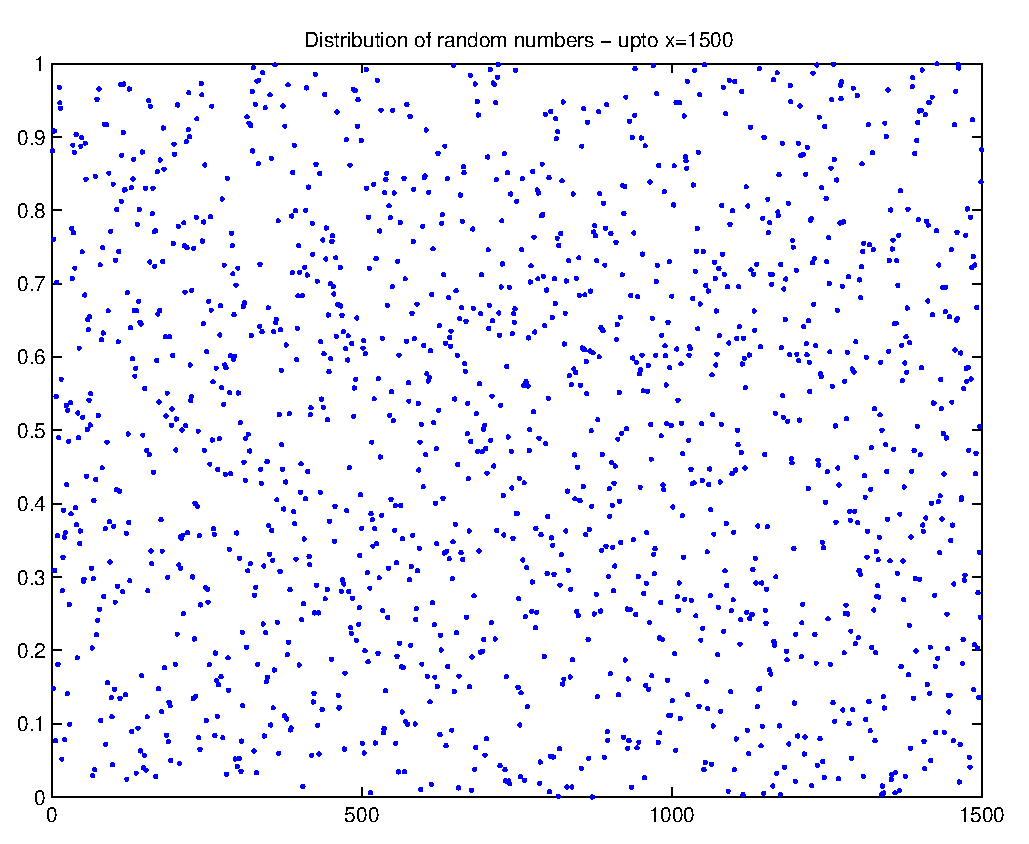
\includegraphics[width=0.95\textwidth]{RandomDistribution}
  \end{center}
  \caption{Distribution of random numbers}
  \label{CHAPTER3_FIG01}
\end{figure}

In mel modo dicam vocibus, eruditi consectetuer vim no, cu quaestio 
instructior eum. Justo nostrud fuisset ea mea, eam an libris repudiandae 
vituperatoribus. Est choro corrumpit definitionem at. Vel sint adhuc vocibus 
ea, illud epicuri eos no. Sea simul officiis ea, et qui veri invidunt 
appellantur. Vix et eros ancillae pertinax.
\begin{equation}
  d\nu_v \;=\; \frac{N}{V}\;\pi\;
               \left(\frac{m}{2\pi\:kT} \right)^{3/2}\;
               v^3\;e^{-mv^2/2kT}\;dv
  \label{CHAPTER3_EQN02}
\end{equation}

Aliquip lobortis ei est, at error viris graeco sed. Vel te elitr detracto, 
modo graecis scripserit ex nec. Errem utamur viderer per no, eam ea eripuit 
referrentur. Pro te dicat disputando.

\begin{table}[hbt]
  \caption{Measured data points representing the relationship between $x$ and
    $y$}
  \begin{center}
    \begin{tabular}{r|rrrrrrrrrrr}
      \hline
      $x$ & 0 & 1 & 2 & 3 & 4 & 5 & 6 & 7 & 8 & 9 & 10\\
      \hline
      $y$ & 0 & 0.94 & 0.99 & -0.52 & -1.82 & -0.44 & 3.54 & 6.69 & 5.38 & 0.00 & -4.42\\
      \hline
    \end{tabular}
  \end{center}
  \label{CHAPTER3_TABLE01}
\end{table}

Et mei mollis scripta, et vim labores phaedrum, in cum facete saperet. 
Splendide elaboraret comprehensam qui ne. Putant verterem no vim, mea solum 
veritus definitiones ei, no labitur propriae deseruisse est. Ius illud everti 
salutandi id, eu facer pericula principes est.

\begin{landscape}
  \begin{table}[hbt]
    \caption{A landscape table: 
      first column represents the year in which the Nobel prize in 
      physics was awarded; second column indicates the name of the 
      scientist and the third column is an \textsl{as is} Nobel
      citation}
    \begin{center}
      \begin{tabular}{p{0.40in}p{2.30in}p{4.85in}}
        \hline
        \multicolumn{1}{c}{\textbf{Year}} &
        \multicolumn{1}{c}{\textbf{Scientist(s)}} &
        \multicolumn{1}{c}{\textbf{Nobel Work}}\\
        \hline
        1901 & W. C. R\"{o}ntgen           & in recognition of the extraordinary services he has rendered by the discovery of the remarkable rays subsequently named after him\\
        1902 & H. A. Lorentz and P. Zeeman & in recognition of the extraordinary service they rendered by their researches into the influence of magnetism upon radiation phenomena\\
        1903 & A. H. Becquerel             & in recognition of the extraordinary services he has rendered by his discovery of spontaneous radioactivity\\
             & M. Curie and P. Curie       & in recognition of the extraordinary services they have rendered by their joint researches on the radiation phenomena discovered by Prof. Henri Becquerel\\
        1904 & J. W. Strutt                & for his investigations of the densities of the most important gases and for his discover argon in connection with these studies\\
        1905 & P. E. A. von Lenard         & Cathode rays\\
        1906 & J. J. Thomson               & Electrical conductivity of gases\\
        1907 & A. A. Michelson             & Spectroscopic and metrological investigations\\
        1908 & G. Lippmann                 & Photographic reproduction of colours\\
        1909 & K. F. Braun and G. Marconi  & Wireless telegraphy\\
        1910 & J. D. van der Waals         & Equation of state of gases and liquids\\
        1911 & W. Wien                     & Laws governing heat radiation\\
        1912 & N. G. Dal\`{e}n             & Automatic regulators for lighting coastal beacons and light buoys\\
        \hline
      \end{tabular}
      \label{CHAPTER3_TABLE02}
    \end{center}
  \end{table}
\end{landscape}

Et mei mollis scripta, et vim labores phaedrum, in cum facete saperet. 
Splendide elaboraret comprehensam qui ne. Putant verterem no vim, mea solum 
veritus definitiones ei, no labitur propriae deseruisse est. Ius illud everti 
salutandi id, eu facer pericula principes est.

\begin{figure}[htb]
  \begin{center}
    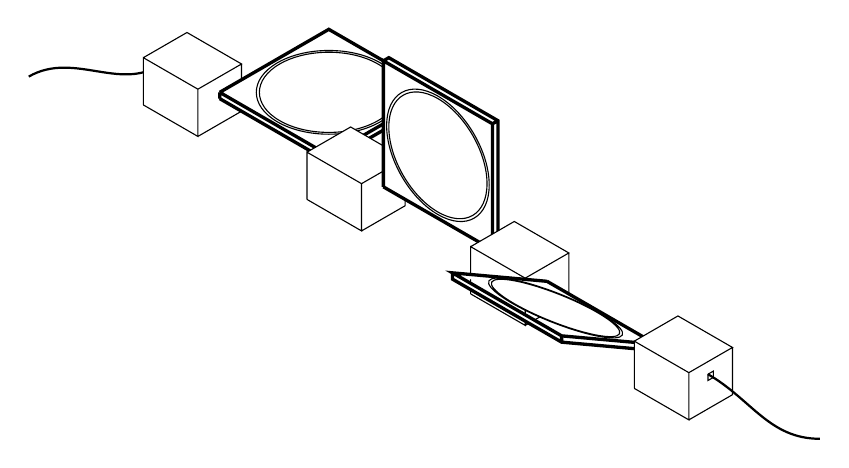
\begin{tikzpicture}[x={(0.866cm,-0.5cm)},
      y={(0.866cm,0.5cm)}, z={(0cm,1cm)}, scale=0.80]
      \tikzstyle{paddle}=[very thick, fill=white]
      \coordinate (O) at (0, 0, 0);

      % fiber in
      \draw[thick] (0,-1.5,0) to[out=30,in=220] (1,0,0);

      % first divider
      \draw[fill=white] (1,-.4,-.5) -- (2,-.4,-.5) -- (2,-.4,.25) --
        (1,-.4,.25) -- (1,-.4,-.5)
        (2,-.4,.25) -- (2,.4,.25) -- (1,.4,.25) -- (1,-.4,.25)
        (2,.4,.25) -- (2,.4,-.5) -- (2,-.4,-.5);

      % first paddle
      \draw[paddle]
        (2,0,0) -- (4,0,0) -- (4,2,0) -- (2,2,0) -- (2,0,0) % first face
        (2,0,0) -- (2,0,-.1)
        (4,0,0) -- (4,0,-.1)
        (2,0,-.1) -- (4,0,-.1) -- (4,2,-.1);
      \draw (3,1,0) circle (.94)
        (3,1,0) circle (.9);

      % second divider
      \draw[fill=white] (4,-.4,-.5) -- (5,-.4,-.5) -- (5,-.4,.25) --
        (4,-.4,.25) -- (4,-.4,-.5)
        (5,-.4,.25) -- (5,.4,.25) -- (4,.4,.25) -- (4,-.4,.25)
        (5,.4,.25) -- (5,.4,-.5) -- (5,-.4,-.5);

      % second paddle
      \filldraw[paddle]
        (5,0,0) -- (7,0,0) -- (7,0,2) -- (5,0,2) -- (5,0,0) % first face
        (7,0,0) -- (7,.1,0) -- (7,.1,2) -- (5,.1,2) -- (5,0,2)
        (7,.1,2) -- (7,0,2);

      % third divider
      \draw[fill=white] (7,-.4,-.5) -- (8,-.4,-.5) -- (8,-.4,.25) --
        (7,-.4,.25) -- (7,-.4,-.5)
        (8,-.4,.25) -- (8,.4,.25) -- (7,.4,.25) -- (7,-.4,.25)
        (8,.4,.25) -- (8,.4,-.5) -- (8,-.4,-.5);

      % third paddle
      \filldraw[paddle]
        (8,0,0) -- (10,0,0) -- (10, -1.732,1) -- (8,-1.732,1) -- (8,0,0)
        (8,-1.732,1) -- (8,-1.732,.9) -- (10,-1.732,.9) -- (10,0,-.1) -- (10,0,0)
        (10,-1.732,.9) -- (10,-1.732,1);

      % fourth divider  
      \draw[fill=white] (10,-.4,-.5) -- (11,-.4,-.5) -- (11,-.4,.25) --
        (10,-.4,.25) -- (10,-.4,-.5)
        (11,-.4,.25) -- (11,.4,.25) -- (10,.4,.25) -- (10,-.4,.25)
        (11,.4,.25) -- (11,.4,-.5) -- (11,-.4,-.5);

      \begin{scope}[x={(0.866cm,-0.5cm)},y={(0,1cm)}]
        \draw (6,0,1) circle (.94)
              (6,0,1) circle (.9);
      \end{scope}
      \begin{scope}[x={(0.866cm,-0.5cm)},y={(-.73cm,.077cm)}]
        \draw[fill=white] (9,1) circle (.94)
          (9,1) circle (.9);
      \end{scope}

      % fiber exit
      \draw (11,-.05,.05) -- (11,.05,.05) --
        (11,.05,-.05) -- (11,-.05,-.05) -- (11,-.05,.05);
      \draw[thick] (10.95,0,0) to[out=-30,in=180] (12,1,-1);
    \end{tikzpicture}
  \end{center}
  \caption{Fibre optics}
  \label{CHAPTER3_FIG01}
\end{figure}

Simul noster voluptaria eam ei, sint regione pri ei. Cum no utinam equidem, 
falli bonorum prodesset an qui. Alterum dissentiet vituperatoribus te eam, 
eos ea suas oblique. Per ea utinam facilisi. Docendi eligendi sit et, pri ea 
dicam eligendi percipitur, has soleat dolores convenire te.

Adipisci molestiae vim at, eum everti accommodare eu. Duo ex maiorum 
consetetur. Sea et vivendo concludaturque, rebum conclusionemque pro eu. Mei 
an everti dolorem. Per id alterum mandamus deseruisse. Copiosae evertitur eum 
ea, atqui interesset est in. Vim magna munere nostrum an, cu congue equidem 
est. Mediocrem reformidans ne mel. Et summo nihil mel, an nam postea 
incorrupte.

In amet verear evertitur qui, ex mea vivendo hendrerit. Ad posse perfecto 
prodesset usu, cum fugit accumsan no. Tempor nonumes duo ea, oblique fabulas 
salutatus ne vis. Ne eam scripta dolorem, graece eruditi eum ei. Ei sed brute 
zril nostro, nostro voluptatum id sea, courtesy of Wikipedia. \cite{Wikipedia}
Adipisci molestiae vim at, eum everti accommodare eu. Duo ex maiorum 
consetetur. Sea et vivendo concludaturque, rebum conclusionemque pro eu.

Adipisci molestiae vim at, eum everti accommodare eu. Duo ex maiorum 
consetetur. Sea et vivendo concludaturque, rebum conclusionemque pro eu. Mei 
an everti dolorem. Per id alterum mandamus deseruisse. Copiosae evertitur eum 
ea, atqui interesset est in. Vim magna munere nostrum an, cu congue equidem 
est. Mediocrem reformidans ne mel. Et summo nihil mel, an nam postea 
incorrupte an everti dolorem. Per id alterum mandamus deseruisse. Copiosae 
evertitur eum ea, atqui interesset est in. Vim magna munere nostrum an, cu 
congue equidem est. Mediocrem reformidans ne mel. Et summo nihil mel, an nam 
postea incorrupte. Mediocrem reformidans ne mel. Et summo nihil mel, an nam 
postea incorrupte an everti dolorem. 

Per id alterum mandamus deseruisse. Copiosae evertitur eum ea, atqui 
interesset est in. Vim magna munere nostrum an, cu congue equidem est. 
Mediocrem reformidans ne mel. Et summo nihil mel, an nam postea incorrupte.

\begin{landscape}
  \begin{figure}[hbt]
    \begin{center}
      \includegraphics[height=4.25in]{TurboProp}
    \end{center}
    \vspace{0.10in}
    \caption{A landscape view of a Turboprop engine - these are 
      jet engine derivatives, still gas turbines, that extract 
      work from the hot-exhaust jet to turn a rotating shaft, 
      which is then used to produce thrust by some other means}
    \label{CHAPTER3_FIG03}
  \end{figure}
\end{landscape}

Id ius soluta semper audiam, ad eos scriptorem concludaturque, id mel rebum 
volumus deserunt. Mel libris percipit scriptorem te, his an dicat putent 
menandri, mazim officiis aliquando mei no. Ne clita veniam disputando vim, 
postea hendrerit maiestatis qui id. Mei te suscipit quaerendum, an aliquando 
intellegebat ius, ei simul detraxit dissentiet eam. Zril dolor ut usu.

Everti saperet vis ut. Scripta maluisset mel eu, duis antiopam in pro. Sea 
diceret contentiones ea. Nec eu duis efficiantur, evertitur constituam 
mediocritatem te vis, pro error regione ad. Sit malorum aliquam at, pericula 
dissentias mei ei. Cu soluta urbanitas est, albucius vituperatoribus usu et.
